\documentclass[1p]{elsarticle_modified}
%\bibliographystyle{elsarticle-num}

%\usepackage[colorlinks]{hyperref}
%\usepackage{abbrmath_seonhwa} %\Abb, \Ascr, \Acal ,\Abf, \Afrak
\usepackage{amsfonts}
\usepackage{amssymb}
\usepackage{amsmath}
\usepackage{amsthm}
\usepackage{scalefnt}
\usepackage{amsbsy}
\usepackage{kotex}
\usepackage{caption}
\usepackage{subfig}
\usepackage{color}
\usepackage{graphicx}
\usepackage{xcolor} %% white, black, red, green, blue, cyan, magenta, yellow
\usepackage{float}
\usepackage{setspace}
\usepackage{hyperref}

\usepackage{tikz}
\usetikzlibrary{arrows}

\usepackage{multirow}
\usepackage{array} % fixed length table
\usepackage{hhline}

%%%%%%%%%%%%%%%%%%%%%
\makeatletter
\renewcommand*\env@matrix[1][\arraystretch]{%
	\edef\arraystretch{#1}%
	\hskip -\arraycolsep
	\let\@ifnextchar\new@ifnextchar
	\array{*\c@MaxMatrixCols c}}
\makeatother %https://tex.stackexchange.com/questions/14071/how-can-i-increase-the-line-spacing-in-a-matrix
%%%%%%%%%%%%%%%

\usepackage[normalem]{ulem}

\newcommand{\msout}[1]{\ifmmode\text{\sout{\ensuremath{#1}}}\else\sout{#1}\fi}
%SOURCE: \msout is \stkout macro in https://tex.stackexchange.com/questions/20609/strikeout-in-math-mode

\newcommand{\cancel}[1]{
	\ifmmode
	{\color{red}\msout{#1}}
	\else
	{\color{red}\sout{#1}}
	\fi
}

\newcommand{\add}[1]{
	{\color{blue}\uwave{#1}}
}

\newcommand{\replace}[2]{
	\ifmmode
	{\color{red}\msout{#1}}{\color{blue}\uwave{#2}}
	\else
	{\color{red}\sout{#1}}{\color{blue}\uwave{#2}}
	\fi
}

\newcommand{\Sol}{\mathcal{S}} %segment
\newcommand{\D}{D} %diagram
\newcommand{\A}{\mathcal{A}} %arc


%%%%%%%%%%%%%%%%%%%%%%%%%%%%%5 test

\def\sl{\operatorname{\textup{SL}}(2,\Cbb)}
\def\psl{\operatorname{\textup{PSL}}(2,\Cbb)}
\def\quan{\mkern 1mu \triangleright \mkern 1mu}

\theoremstyle{definition}
\newtheorem{thm}{Theorem}[section]
\newtheorem{prop}[thm]{Proposition}
\newtheorem{lem}[thm]{Lemma}
\newtheorem{ques}[thm]{Question}
\newtheorem{cor}[thm]{Corollary}
\newtheorem{defn}[thm]{Definition}
\newtheorem{exam}[thm]{Example}
\newtheorem{rmk}[thm]{Remark}
\newtheorem{alg}[thm]{Algorithm}

\newcommand{\I}{\sqrt{-1}}
\begin{document}

%\begin{frontmatter}
%
%\title{Boundary parabolic representations of knots up to 8 crossings}
%
%%% Group authors per affiliation:
%\author{Yunhi Cho} 
%\address{Department of Mathematics, University of Seoul, Seoul, Korea}
%\ead{yhcho@uos.ac.kr}
%
%
%\author{Seonhwa Kim} %\fnref{s_kim}}
%\address{Center for Geometry and Physics, Institute for Basic Science, Pohang, 37673, Korea}
%\ead{ryeona17@ibs.re.kr}
%
%\author{Hyuk Kim}
%\address{Department of Mathematical Sciences, Seoul National University, Seoul 08826, Korea}
%\ead{hyukkim@snu.ac.kr}
%
%\author{Seokbeom Yoon}
%\address{Department of Mathematical Sciences, Seoul National University, Seoul, 08826,  Korea}
%\ead{sbyoon15@snu.ac.kr}
%
%\begin{abstract}
%We find all boundary parabolic representation of knots up to 8 crossings.
%
%\end{abstract}
%\begin{keyword}
%    \MSC[2010] 57M25 
%\end{keyword}
%
%\end{frontmatter}

%\linenumbers
%\tableofcontents
%
\newcommand\colored[1]{\textcolor{white}{\rule[-0.35ex]{0.8em}{1.4ex}}\kern-0.8em\color{red} #1}%
%\newcommand\colored[1]{\textcolor{white}{ #1}\kern-2.17ex	\textcolor{white}{ #1}\kern-1.81ex	\textcolor{white}{ #1}\kern-2.15ex\color{red}#1	}

{\Large $\underline{12n_{0724}~(K12n_{0724})}$}

\setlength{\tabcolsep}{10pt}
\renewcommand{\arraystretch}{1.6}
\vspace{1cm}\begin{tabular}{m{100pt}>{\centering\arraybackslash}m{274pt}}
\multirow{5}{120pt}{
	\centering
	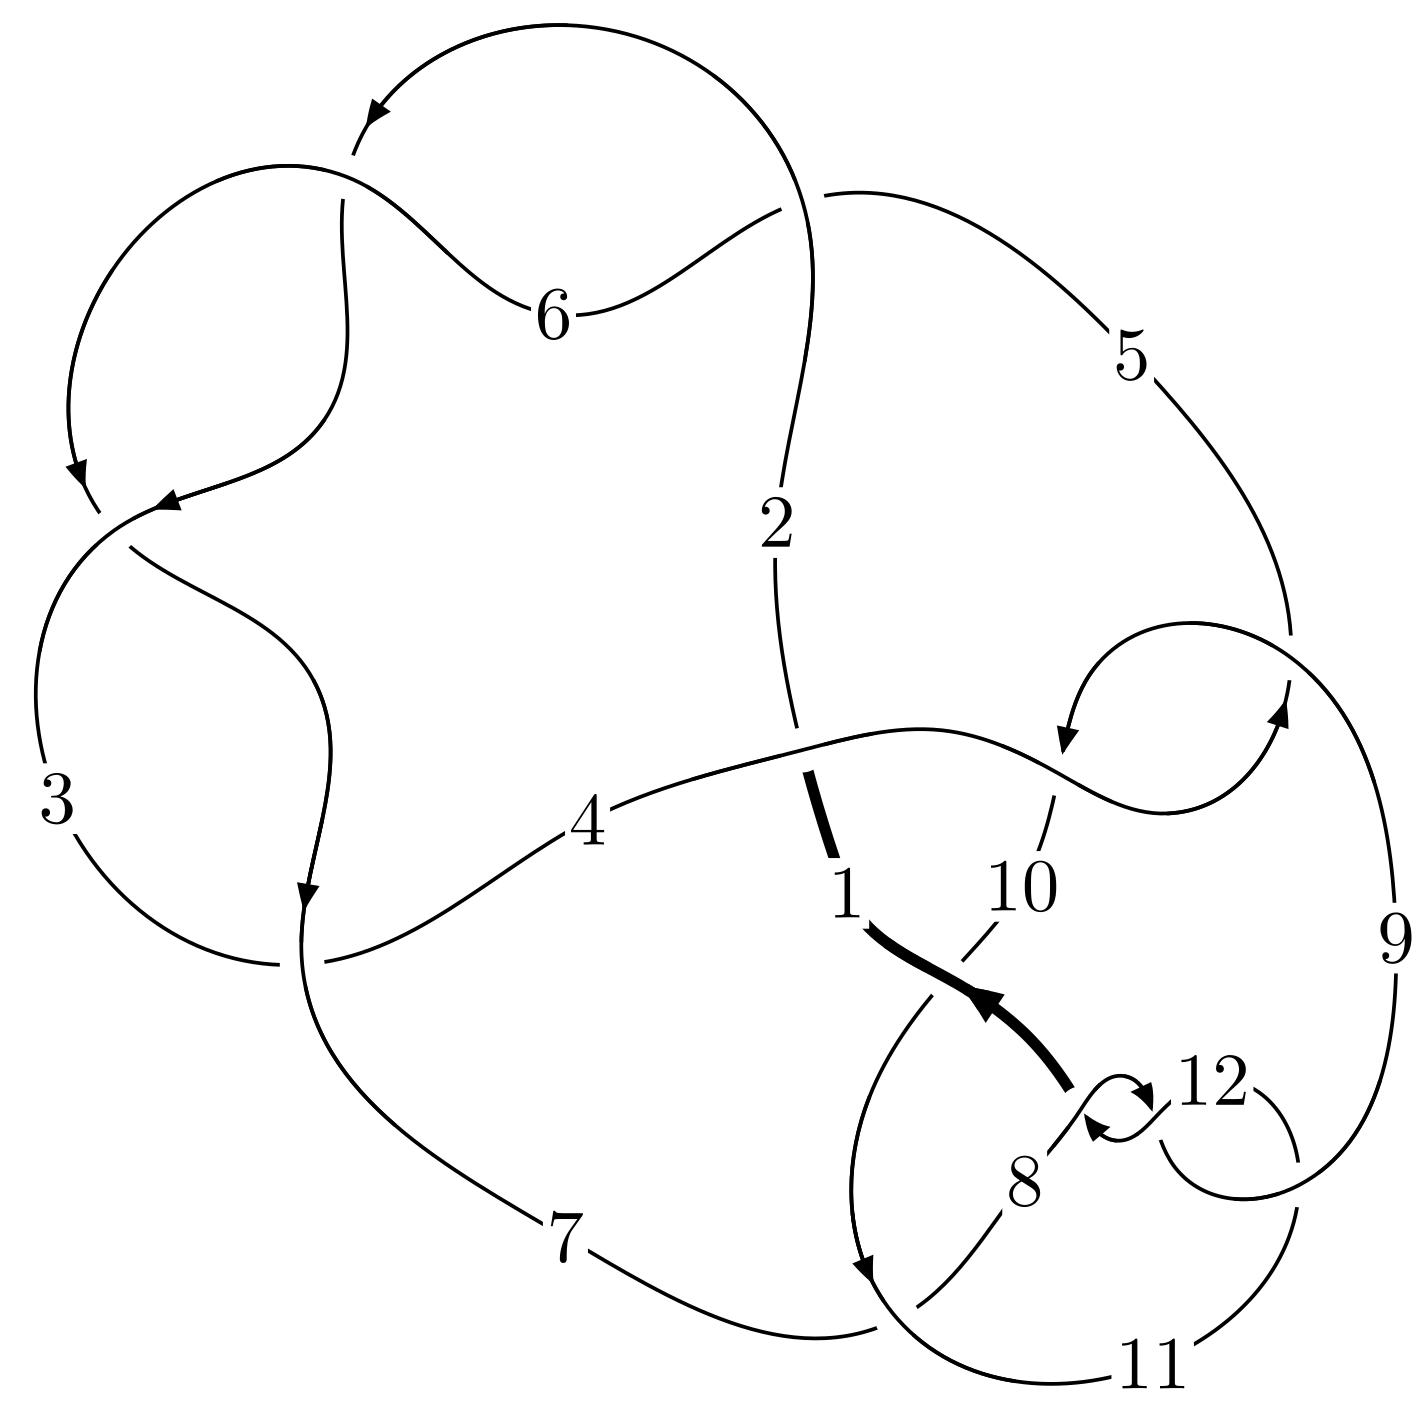
\includegraphics[width=112pt]{../../../GIT/diagram.site/Diagrams/png/2813_12n_0724.png}\\
\ \ \ A knot diagram\footnotemark}&
\allowdisplaybreaks
\textbf{Linearized knot diagam} \\
\cline{2-2}
 &
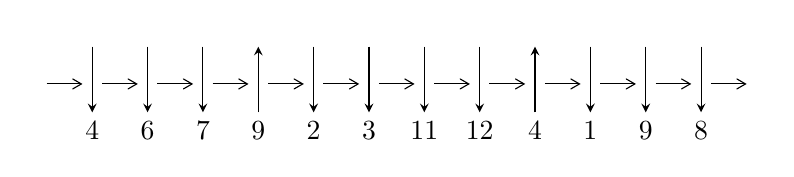
\begin{tikzpicture}[x=20pt, y=17pt]
	% nodes
	\node (C0) at (0, 0) {};
	\node (C1) at (1, 0) {};
	\node (C1U) at (1, +1) {};
	\node (C1D) at (1, -1) {4};

	\node (C2) at (2, 0) {};
	\node (C2U) at (2, +1) {};
	\node (C2D) at (2, -1) {6};

	\node (C3) at (3, 0) {};
	\node (C3U) at (3, +1) {};
	\node (C3D) at (3, -1) {7};

	\node (C4) at (4, 0) {};
	\node (C4U) at (4, +1) {};
	\node (C4D) at (4, -1) {9};

	\node (C5) at (5, 0) {};
	\node (C5U) at (5, +1) {};
	\node (C5D) at (5, -1) {2};

	\node (C6) at (6, 0) {};
	\node (C6U) at (6, +1) {};
	\node (C6D) at (6, -1) {3};

	\node (C7) at (7, 0) {};
	\node (C7U) at (7, +1) {};
	\node (C7D) at (7, -1) {11};

	\node (C8) at (8, 0) {};
	\node (C8U) at (8, +1) {};
	\node (C8D) at (8, -1) {12};

	\node (C9) at (9, 0) {};
	\node (C9U) at (9, +1) {};
	\node (C9D) at (9, -1) {4};

	\node (C10) at (10, 0) {};
	\node (C10U) at (10, +1) {};
	\node (C10D) at (10, -1) {1};

	\node (C11) at (11, 0) {};
	\node (C11U) at (11, +1) {};
	\node (C11D) at (11, -1) {9};

	\node (C12) at (12, 0) {};
	\node (C12U) at (12, +1) {};
	\node (C12D) at (12, -1) {8};
	\node (C13) at (13, 0) {};

	% arrows
	\draw[->,>={angle 60}]
	(C0) edge (C1) (C1) edge (C2) (C2) edge (C3) (C3) edge (C4) (C4) edge (C5) (C5) edge (C6) (C6) edge (C7) (C7) edge (C8) (C8) edge (C9) (C9) edge (C10) (C10) edge (C11) (C11) edge (C12) (C12) edge (C13) ;	\draw[->,>=stealth]
	(C1U) edge (C1D) (C2U) edge (C2D) (C3U) edge (C3D) (C4D) edge (C4U) (C5U) edge (C5D) (C6U) edge (C6D) (C7U) edge (C7D) (C8U) edge (C8D) (C9D) edge (C9U) (C10U) edge (C10D) (C11U) edge (C11D) (C12U) edge (C12D) ;
	\end{tikzpicture} \\
\hhline{~~} \\& 
\textbf{Solving Sequence} \\ \cline{2-2} 
 &
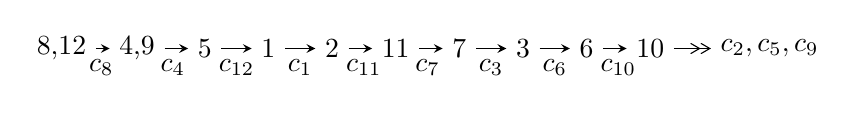
\begin{tikzpicture}[x=23pt, y=7pt]
	% node
	\node (A0) at (-1/8, 0) {8,12};
	\node (A1) at (17/16, 0) {4,9};
	\node (A2) at (17/8, 0) {5};
	\node (A3) at (25/8, 0) {1};
	\node (A4) at (33/8, 0) {2};
	\node (A5) at (41/8, 0) {11};
	\node (A6) at (49/8, 0) {7};
	\node (A7) at (57/8, 0) {3};
	\node (A8) at (65/8, 0) {6};
	\node (A9) at (73/8, 0) {10};
	\node (C1) at (1/2, -1) {$c_{8}$};
	\node (C2) at (13/8, -1) {$c_{4}$};
	\node (C3) at (21/8, -1) {$c_{12}$};
	\node (C4) at (29/8, -1) {$c_{1}$};
	\node (C5) at (37/8, -1) {$c_{11}$};
	\node (C6) at (45/8, -1) {$c_{7}$};
	\node (C7) at (53/8, -1) {$c_{3}$};
	\node (C8) at (61/8, -1) {$c_{6}$};
	\node (C9) at (69/8, -1) {$c_{10}$};
	\node (A10) at (11, 0) {$c_{2},c_{5},c_{9}$};

	% edge
	\draw[->,>=stealth]	
	(A0) edge (A1) (A1) edge (A2) (A2) edge (A3) (A3) edge (A4) (A4) edge (A5) (A5) edge (A6) (A6) edge (A7) (A7) edge (A8) (A8) edge (A9) ;
	\draw[->>,>={angle 60}]	
	(A9) edge (A10);
\end{tikzpicture} \\ 

\end{tabular} \\

\footnotetext{
The image of knot diagram is generated by the software ``\textbf{Draw programme}" developed by Andrew Bartholomew(\url{http://www.layer8.co.uk/maths/draw/index.htm\#Running-draw}), where we modified some parts for our purpose(\url{https://github.com/CATsTAILs/LinksPainter}).
}\phantom \\ \newline 
\centering \textbf{Ideals for irreducible components\footnotemark of $X_{\text{par}}$} 
 
\begin{align*}
I^u_{1}&=\langle 
- u^{34}-2 u^{33}+\cdots+2 b+2,\;3 u^{35}+9 u^{34}+\cdots+2 a+12,\;u^{36}+3 u^{35}+\cdots+5 u+1\rangle \\
I^u_{2}&=\langle 
- u^2 a+b,\;- u^2 a+a^2- u^2- a+u-2,\;u^3- u^2+2 u-1\rangle \\
\\
\end{align*}
\raggedright * 2 irreducible components of $\dim_{\mathbb{C}}=0$, with total 42 representations.\\
\footnotetext{All coefficients of polynomials are rational numbers. But the coefficients are sometimes approximated in decimal forms when there is not enough margin.}
\newpage
\renewcommand{\arraystretch}{1}
\centering \section*{I. $I^u_{1}= \langle - u^{34}-2 u^{33}+\cdots+2 b+2,\;3 u^{35}+9 u^{34}+\cdots+2 a+12,\;u^{36}+3 u^{35}+\cdots+5 u+1 \rangle$}
\flushleft \textbf{(i) Arc colorings}\\
\begin{tabular}{m{7pt} m{180pt} m{7pt} m{180pt} }
\flushright $a_{8}=$&$\begin{pmatrix}1\\0\end{pmatrix}$ \\
\flushright $a_{12}=$&$\begin{pmatrix}0\\u\end{pmatrix}$ \\
\flushright $a_{4}=$&$\begin{pmatrix}-\frac{3}{2} u^{35}-\frac{9}{2} u^{34}+\cdots-\frac{13}{2} u-6\\\frac{1}{2} u^{34}+u^{33}+\cdots+\frac{1}{2} u-1\end{pmatrix}$ \\
\flushright $a_{9}=$&$\begin{pmatrix}1\\u^2\end{pmatrix}$ \\
\flushright $a_{5}=$&$\begin{pmatrix}-\frac{3}{2} u^{35}-\frac{9}{2} u^{34}+\cdots-\frac{15}{2} u-7\\-\frac{1}{2} u^{34}- u^{33}+\cdots+\frac{1}{2} u-1\end{pmatrix}$ \\
\flushright $a_{1}=$&$\begin{pmatrix}- u\\u\end{pmatrix}$ \\
\flushright $a_{2}=$&$\begin{pmatrix}-\frac{1}{2} u^{35}-\frac{3}{2} u^{34}+\cdots+12 u^2-\frac{15}{2} u\\\frac{1}{2} u^{34}+u^{33}+\cdots+\frac{9}{2} u^2+\frac{1}{2} u\end{pmatrix}$ \\
\flushright $a_{11}=$&$\begin{pmatrix}u\\u^3+u\end{pmatrix}$ \\
\flushright $a_{7}=$&$\begin{pmatrix}- u^4- u^2+1\\- u^6-2 u^4- u^2\end{pmatrix}$ \\
\flushright $a_{3}=$&$\begin{pmatrix}-2 u^{35}-6 u^{34}+\cdots-\frac{25}{2} u-\frac{17}{2}\\-\frac{3}{2} u^{35}-2 u^{34}+\cdots+\frac{3}{2} u-\frac{1}{2}\end{pmatrix}$ \\
\flushright $a_{6}=$&$\begin{pmatrix}u^{35}+3 u^{34}+\cdots+\frac{19}{2} u+\frac{3}{2}\\-\frac{1}{2} u^{35}-2 u^{34}+\cdots-\frac{3}{2} u-\frac{1}{2}\end{pmatrix}$ \\
\flushright $a_{10}=$&$\begin{pmatrix}u^5+2 u^3+u\\- u^5- u^3+u\end{pmatrix}$\\&\end{tabular}
\flushleft \textbf{(ii) Obstruction class $= -1$}\\~\\
\flushleft \textbf{(iii) Cusp Shapes $= - u^{35}-\frac{5}{2} u^{34}+\cdots-12 u-\frac{21}{2}$}\\~\\
\newpage\renewcommand{\arraystretch}{1}
\flushleft \textbf{(iv) u-Polynomials at the component}\newline \\
\begin{tabular}{m{50pt}|m{274pt}}
Crossings & \hspace{64pt}u-Polynomials at each crossing \\
\hline $$\begin{aligned}c_{1}\end{aligned}$$&$\begin{aligned}
&u^{36}-4 u^{35}+\cdots+4 u+1
\end{aligned}$\\
\hline $$\begin{aligned}c_{2},c_{3},c_{5}\\c_{6}\end{aligned}$$&$\begin{aligned}
&u^{36}+4 u^{35}+\cdots-2 u+1
\end{aligned}$\\
\hline $$\begin{aligned}c_{4},c_{9}\end{aligned}$$&$\begin{aligned}
&u^{36}+u^{35}+\cdots+32 u+64
\end{aligned}$\\
\hline $$\begin{aligned}c_{7}\end{aligned}$$&$\begin{aligned}
&u^{36}+3 u^{35}+\cdots-905 u+241
\end{aligned}$\\
\hline $$\begin{aligned}c_{8},c_{11},c_{12}\end{aligned}$$&$\begin{aligned}
&u^{36}-3 u^{35}+\cdots-5 u+1
\end{aligned}$\\
\hline $$\begin{aligned}c_{10}\end{aligned}$$&$\begin{aligned}
&u^{36}-5 u^{35}+\cdots+9 u+3
\end{aligned}$\\
\hline
\end{tabular}\\~\\
\newpage\renewcommand{\arraystretch}{1}
\flushleft \textbf{(v) Riley Polynomials at the component}\newline \\
\begin{tabular}{m{50pt}|m{274pt}}
Crossings & \hspace{64pt}Riley Polynomials at each crossing \\
\hline $$\begin{aligned}c_{1}\end{aligned}$$&$\begin{aligned}
&y^{36}+44 y^{35}+\cdots-26 y+1
\end{aligned}$\\
\hline $$\begin{aligned}c_{2},c_{3},c_{5}\\c_{6}\end{aligned}$$&$\begin{aligned}
&y^{36}-40 y^{35}+\cdots-26 y+1
\end{aligned}$\\
\hline $$\begin{aligned}c_{4},c_{9}\end{aligned}$$&$\begin{aligned}
&y^{36}-35 y^{35}+\cdots-82944 y+4096
\end{aligned}$\\
\hline $$\begin{aligned}c_{7}\end{aligned}$$&$\begin{aligned}
&y^{36}+15 y^{35}+\cdots-1047493 y+58081
\end{aligned}$\\
\hline $$\begin{aligned}c_{8},c_{11},c_{12}\end{aligned}$$&$\begin{aligned}
&y^{36}+35 y^{35}+\cdots-29 y+1
\end{aligned}$\\
\hline $$\begin{aligned}c_{10}\end{aligned}$$&$\begin{aligned}
&y^{36}+35 y^{35}+\cdots-885 y+9
\end{aligned}$\\
\hline
\end{tabular}\\~\\
\newpage\flushleft \textbf{(vi) Complex Volumes and Cusp Shapes}
$$\begin{array}{c|c|c}  
\text{Solutions to }I^u_{1}& \I (\text{vol} + \sqrt{-1}CS) & \text{Cusp shape}\\
 \hline 
\begin{aligned}
u &= -0.584918 + 0.622459 I \\
a &= -0.393281 + 0.608399 I \\
b &= -1.024860 + 0.631550 I\end{aligned}
 & -1.06074 - 3.44814 I & -9.28468 + 0.39535 I \\ \hline\begin{aligned}
u &= -0.584918 - 0.622459 I \\
a &= -0.393281 - 0.608399 I \\
b &= -1.024860 - 0.631550 I\end{aligned}
 & -1.06074 + 3.44814 I & -9.28468 - 0.39535 I \\ \hline\begin{aligned}
u &= -0.750111 + 0.395247 I \\
a &= \phantom{-}0.51873 - 1.46690 I \\
b &= \phantom{-}0.823106 - 0.363879 I\end{aligned}
 & -1.86419 + 7.98474 I & -10.81435 - 5.76584 I \\ \hline\begin{aligned}
u &= -0.750111 - 0.395247 I \\
a &= \phantom{-}0.51873 + 1.46690 I \\
b &= \phantom{-}0.823106 + 0.363879 I\end{aligned}
 & -1.86419 - 7.98474 I & -10.81435 + 5.76584 I \\ \hline\begin{aligned}
u &= -0.704933 + 0.458093 I \\
a &= -0.514731 + 1.219340 I \\
b &= -0.898045 + 0.419560 I\end{aligned}
 & \phantom{-}5.07187 + 4.59949 I & -7.09710 - 5.90387 I \\ \hline\begin{aligned}
u &= -0.704933 - 0.458093 I \\
a &= -0.514731 - 1.219340 I \\
b &= -0.898045 - 0.419560 I\end{aligned}
 & \phantom{-}5.07187 - 4.59949 I & -7.09710 + 5.90387 I \\ \hline\begin{aligned}
u &= -0.650250 + 0.527342 I \\
a &= \phantom{-}0.486347 - 0.943180 I \\
b &= \phantom{-}0.959920 - 0.500736 I\end{aligned}
 & \phantom{-}5.33026 - 0.08250 I & -6.15458 - 0.14164 I \\ \hline\begin{aligned}
u &= -0.650250 - 0.527342 I \\
a &= \phantom{-}0.486347 + 0.943180 I \\
b &= \phantom{-}0.959920 + 0.500736 I\end{aligned}
 & \phantom{-}5.33026 + 0.08250 I & -6.15458 + 0.14164 I \\ \hline\begin{aligned}
u &= \phantom{-}0.781619\phantom{ +0.000000I} \\
a &= -0.928457\phantom{ +0.000000I} \\
b &= \phantom{-}0.540395\phantom{ +0.000000I}\end{aligned}
 & -7.32938\phantom{ +0.000000I} & -12.6770\phantom{ +0.000000I} \\ \hline\begin{aligned}
u &= \phantom{-}0.333725 + 1.215310 I \\
a &= -0.313201 - 0.777608 I \\
b &= -0.067999 + 0.938160 I\end{aligned}
 & -3.58469 - 4.02994 I & -8.71251 + 3.82957 I\\
 \hline 
 \end{array}$$\newpage$$\begin{array}{c|c|c}  
\text{Solutions to }I^u_{1}& \I (\text{vol} + \sqrt{-1}CS) & \text{Cusp shape}\\
 \hline 
\begin{aligned}
u &= \phantom{-}0.333725 - 1.215310 I \\
a &= -0.313201 + 0.777608 I \\
b &= -0.067999 - 0.938160 I\end{aligned}
 & -3.58469 + 4.02994 I & -8.71251 - 3.82957 I \\ \hline\begin{aligned}
u &= \phantom{-}0.239600 + 1.278530 I \\
a &= \phantom{-}0.185138 + 0.409163 I \\
b &= \phantom{-}0.007593 - 0.541465 I\end{aligned}
 & \phantom{-}2.51540 - 3.15546 I & \phantom{-}0.55293 + 6.85711 I \\ \hline\begin{aligned}
u &= \phantom{-}0.239600 - 1.278530 I \\
a &= \phantom{-}0.185138 - 0.409163 I \\
b &= \phantom{-}0.007593 + 0.541465 I\end{aligned}
 & \phantom{-}2.51540 + 3.15546 I & \phantom{-}0.55293 - 6.85711 I \\ \hline\begin{aligned}
u &= \phantom{-}0.570266 + 0.400726 I \\
a &= -0.877489 - 0.756539 I \\
b &= \phantom{-}0.297801 + 0.607076 I\end{aligned}
 & -6.37924 - 1.83035 I & -12.43917 + 3.59444 I \\ \hline\begin{aligned}
u &= \phantom{-}0.570266 - 0.400726 I \\
a &= -0.877489 + 0.756539 I \\
b &= \phantom{-}0.297801 - 0.607076 I\end{aligned}
 & -6.37924 + 1.83035 I & -12.43917 - 3.59444 I \\ \hline\begin{aligned}
u &= -0.096640 + 1.314140 I \\
a &= -1.86833 - 0.54003 I \\
b &= \phantom{-}2.39929 + 1.89454 I\end{aligned}
 & -5.49210 + 1.78793 I & -8.00000 + 1.75055 I \\ \hline\begin{aligned}
u &= -0.096640 - 1.314140 I \\
a &= -1.86833 + 0.54003 I \\
b &= \phantom{-}2.39929 - 1.89454 I\end{aligned}
 & -5.49210 - 1.78793 I & -8.00000 - 1.75055 I \\ \hline\begin{aligned}
u &= \phantom{-}0.003093 + 1.351590 I \\
a &= \phantom{-}1.346750 + 0.048804 I \\
b &= -1.75931 - 0.78922 I\end{aligned}
 & \phantom{-}2.91594 + 0.49680 I & -6.76015 - 1.46543 I \\ \hline\begin{aligned}
u &= \phantom{-}0.003093 - 1.351590 I \\
a &= \phantom{-}1.346750 - 0.048804 I \\
b &= -1.75931 + 0.78922 I\end{aligned}
 & \phantom{-}2.91594 - 0.49680 I & -6.76015 + 1.46543 I \\ \hline\begin{aligned}
u &= \phantom{-}0.632707\phantom{ +0.000000I} \\
a &= \phantom{-}0.514711\phantom{ +0.000000I} \\
b &= -0.261536\phantom{ +0.000000I}\end{aligned}
 & -1.47548\phantom{ +0.000000I} & -4.26650\phantom{ +0.000000I}\\
 \hline 
 \end{array}$$\newpage$$\begin{array}{c|c|c}  
\text{Solutions to }I^u_{1}& \I (\text{vol} + \sqrt{-1}CS) & \text{Cusp shape}\\
 \hline 
\begin{aligned}
u &= \phantom{-}0.118075 + 1.391920 I \\
a &= -0.902722 + 0.302362 I \\
b &= \phantom{-}1.248310 + 0.060515 I\end{aligned}
 & \phantom{-}4.66390 - 2.61771 I & -2.92989 + 4.33183 I \\ \hline\begin{aligned}
u &= \phantom{-}0.118075 - 1.391920 I \\
a &= -0.902722 - 0.302362 I \\
b &= \phantom{-}1.248310 - 0.060515 I\end{aligned}
 & \phantom{-}4.66390 + 2.61771 I & -2.92989 - 4.33183 I \\ \hline\begin{aligned}
u &= \phantom{-}0.20804 + 1.44313 I \\
a &= \phantom{-}0.670803 - 0.683664 I \\
b &= -1.072410 + 0.518782 I\end{aligned}
 & -0.46527 - 4.68513 I & -8.00000 + 0. I\phantom{ +0.000000I} \\ \hline\begin{aligned}
u &= \phantom{-}0.20804 - 1.44313 I \\
a &= \phantom{-}0.670803 + 0.683664 I \\
b &= -1.072410 - 0.518782 I\end{aligned}
 & -0.46527 + 4.68513 I & -8.00000 + 0. I\phantom{ +0.000000I} \\ \hline\begin{aligned}
u &= -0.28295 + 1.47214 I \\
a &= -2.04519 + 0.99112 I \\
b &= \phantom{-}3.54834 - 1.01341 I\end{aligned}
 & \phantom{-}4.15419 + 11.75140 I & \phantom{-0.000000 } 0 \\ \hline\begin{aligned}
u &= -0.28295 - 1.47214 I \\
a &= -2.04519 - 0.99112 I \\
b &= \phantom{-}3.54834 + 1.01341 I\end{aligned}
 & \phantom{-}4.15419 - 11.75140 I & \phantom{-0.000000 } 0 \\ \hline\begin{aligned}
u &= -0.25376 + 1.49060 I \\
a &= \phantom{-}2.05918 - 0.92299 I \\
b &= -3.47531 + 0.84038 I\end{aligned}
 & \phantom{-}11.38500 + 8.10134 I & \phantom{-0.000000 } 0 \\ \hline\begin{aligned}
u &= -0.25376 - 1.49060 I \\
a &= \phantom{-}2.05918 + 0.92299 I \\
b &= -3.47531 - 0.84038 I\end{aligned}
 & \phantom{-}11.38500 - 8.10134 I & \phantom{-0.000000 } 0 \\ \hline\begin{aligned}
u &= -0.16804 + 1.50765 I \\
a &= \phantom{-}1.98331 - 0.75551 I \\
b &= -3.17021 + 0.44936 I\end{aligned}
 & \phantom{-}5.88626 - 0.82923 I & \phantom{-0.000000 } 0 \\ \hline\begin{aligned}
u &= -0.16804 - 1.50765 I \\
a &= \phantom{-}1.98331 + 0.75551 I \\
b &= -3.17021 - 0.44936 I\end{aligned}
 & \phantom{-}5.88626 + 0.82923 I & \phantom{-0.000000 } 0\\
 \hline 
 \end{array}$$\newpage$$\begin{array}{c|c|c}  
\text{Solutions to }I^u_{1}& \I (\text{vol} + \sqrt{-1}CS) & \text{Cusp shape}\\
 \hline 
\begin{aligned}
u &= -0.21821 + 1.50283 I \\
a &= -2.04552 + 0.85247 I \\
b &= \phantom{-}3.36643 - 0.66614 I\end{aligned}
 & \phantom{-}11.93180 + 3.06807 I & \phantom{-0.000000 } 0 \\ \hline\begin{aligned}
u &= -0.21821 - 1.50283 I \\
a &= -2.04552 - 0.85247 I \\
b &= \phantom{-}3.36643 + 0.66614 I\end{aligned}
 & \phantom{-}11.93180 - 3.06807 I & \phantom{-0.000000 } 0 \\ \hline\begin{aligned}
u &= -0.419044\phantom{ +0.000000I} \\
a &= \phantom{-}3.28668\phantom{ +0.000000I} \\
b &= \phantom{-}1.05760\phantom{ +0.000000I}\end{aligned}
 & -9.57946\phantom{ +0.000000I} & -1.90810\phantom{ +0.000000I} \\ \hline\begin{aligned}
u &= \phantom{-}0.352645 + 0.225056 I \\
a &= \phantom{-}0.666608 + 0.999666 I \\
b &= -0.054962 - 0.463386 I\end{aligned}
 & -0.508387 - 0.873575 I & -8.67347 + 7.93671 I \\ \hline\begin{aligned}
u &= \phantom{-}0.352645 - 0.225056 I \\
a &= \phantom{-}0.666608 - 0.999666 I \\
b &= -0.054962 + 0.463386 I\end{aligned}
 & -0.508387 + 0.873575 I & -8.67347 - 7.93671 I \\ \hline\begin{aligned}
u &= -0.226552\phantom{ +0.000000I} \\
a &= -2.78574\phantom{ +0.000000I} \\
b &= -0.591839\phantom{ +0.000000I}\end{aligned}
 & -1.26761\phantom{ +0.000000I} & -6.33540\phantom{ +0.000000I}\\
 \hline 
 \end{array}$$\newpage\newpage\renewcommand{\arraystretch}{1}
\centering \section*{II. $I^u_{2}= \langle - u^2 a+b,\;- u^2 a+a^2- u^2- a+u-2,\;u^3- u^2+2 u-1 \rangle$}
\flushleft \textbf{(i) Arc colorings}\\
\begin{tabular}{m{7pt} m{180pt} m{7pt} m{180pt} }
\flushright $a_{8}=$&$\begin{pmatrix}1\\0\end{pmatrix}$ \\
\flushright $a_{12}=$&$\begin{pmatrix}0\\u\end{pmatrix}$ \\
\flushright $a_{4}=$&$\begin{pmatrix}a\\u^2 a\end{pmatrix}$ \\
\flushright $a_{9}=$&$\begin{pmatrix}1\\u^2\end{pmatrix}$ \\
\flushright $a_{5}=$&$\begin{pmatrix}a\\u^2 a\end{pmatrix}$ \\
\flushright $a_{1}=$&$\begin{pmatrix}- u\\u\end{pmatrix}$ \\
\flushright $a_{2}=$&$\begin{pmatrix}- u^2- a- u-1\\- u^2 a+2 u-1\end{pmatrix}$ \\
\flushright $a_{11}=$&$\begin{pmatrix}u\\u^2- u+1\end{pmatrix}$ \\
\flushright $a_{7}=$&$\begin{pmatrix}u\\- u\end{pmatrix}$ \\
\flushright $a_{3}=$&$\begin{pmatrix}- a u+2 a\\u^2 a+a u- a\end{pmatrix}$ \\
\flushright $a_{6}=$&$\begin{pmatrix}a u- u^2-2 a-1\\- u^2 a- a u+a+u-1\end{pmatrix}$ \\
\flushright $a_{10}=$&$\begin{pmatrix}1\\u^2\end{pmatrix}$\\&\end{tabular}
\flushleft \textbf{(ii) Obstruction class $= 1$}\\~\\
\flushleft \textbf{(iii) Cusp Shapes $= - u^2 a- a u-5 u^2+3 u-20$}\\~\\
\newpage\renewcommand{\arraystretch}{1}
\flushleft \textbf{(iv) u-Polynomials at the component}\newline \\
\begin{tabular}{m{50pt}|m{274pt}}
Crossings & \hspace{64pt}u-Polynomials at each crossing \\
\hline $$\begin{aligned}c_{1},c_{2},c_{3}\end{aligned}$$&$\begin{aligned}
&(u^2+u-1)^3
\end{aligned}$\\
\hline $$\begin{aligned}c_{4},c_{9}\end{aligned}$$&$\begin{aligned}
&u^6
\end{aligned}$\\
\hline $$\begin{aligned}c_{5},c_{6}\end{aligned}$$&$\begin{aligned}
&(u^2- u-1)^3
\end{aligned}$\\
\hline $$\begin{aligned}c_{7},c_{10}\end{aligned}$$&$\begin{aligned}
&(u^3+u^2-1)^2
\end{aligned}$\\
\hline $$\begin{aligned}c_{8}\end{aligned}$$&$\begin{aligned}
&(u^3- u^2+2 u-1)^2
\end{aligned}$\\
\hline $$\begin{aligned}c_{11},c_{12}\end{aligned}$$&$\begin{aligned}
&(u^3+u^2+2 u+1)^2
\end{aligned}$\\
\hline
\end{tabular}\\~\\
\newpage\renewcommand{\arraystretch}{1}
\flushleft \textbf{(v) Riley Polynomials at the component}\newline \\
\begin{tabular}{m{50pt}|m{274pt}}
Crossings & \hspace{64pt}Riley Polynomials at each crossing \\
\hline $$\begin{aligned}c_{1},c_{2},c_{3}\\c_{5},c_{6}\end{aligned}$$&$\begin{aligned}
&(y^2-3 y+1)^3
\end{aligned}$\\
\hline $$\begin{aligned}c_{4},c_{9}\end{aligned}$$&$\begin{aligned}
&y^6
\end{aligned}$\\
\hline $$\begin{aligned}c_{7},c_{10}\end{aligned}$$&$\begin{aligned}
&(y^3- y^2+2 y-1)^2
\end{aligned}$\\
\hline $$\begin{aligned}c_{8},c_{11},c_{12}\end{aligned}$$&$\begin{aligned}
&(y^3+3 y^2+2 y-1)^2
\end{aligned}$\\
\hline
\end{tabular}\\~\\
\newpage\flushleft \textbf{(vi) Complex Volumes and Cusp Shapes}
$$\begin{array}{c|c|c}  
\text{Solutions to }I^u_{2}& \I (\text{vol} + \sqrt{-1}CS) & \text{Cusp shape}\\
 \hline 
\begin{aligned}
u &= \phantom{-}0.215080 + 1.307140 I \\
a &= -1.071720 + 0.909787 I \\
b &= \phantom{-}1.27003 - 2.11500 I\end{aligned}
 & -5.85852 - 2.82812 I & -10.89327 + 4.43024 I \\ \hline\begin{aligned}
u &= \phantom{-}0.215080 + 1.307140 I \\
a &= \phantom{-}0.409360 - 0.347508 I \\
b &= -0.485107 + 0.807858 I\end{aligned}
 & \phantom{-}2.03717 - 2.82812 I & -11.10015 - 0.15818 I \\ \hline\begin{aligned}
u &= \phantom{-}0.215080 - 1.307140 I \\
a &= -1.071720 - 0.909787 I \\
b &= \phantom{-}1.27003 + 2.11500 I\end{aligned}
 & -5.85852 + 2.82812 I & -10.89327 - 4.43024 I \\ \hline\begin{aligned}
u &= \phantom{-}0.215080 - 1.307140 I \\
a &= \phantom{-}0.409360 + 0.347508 I \\
b &= -0.485107 - 0.807858 I\end{aligned}
 & \phantom{-}2.03717 + 2.82812 I & -11.10015 + 0.15818 I \\ \hline\begin{aligned}
u &= \phantom{-}0.569840\phantom{ +0.000000I} \\
a &= -0.818721\phantom{ +0.000000I} \\
b &= -0.265853\phantom{ +0.000000I}\end{aligned}
 & -2.10041\phantom{ +0.000000I} & -19.1820\phantom{ +0.000000I} \\ \hline\begin{aligned}
u &= \phantom{-}0.569840\phantom{ +0.000000I} \\
a &= \phantom{-}2.14344\phantom{ +0.000000I} \\
b &= \phantom{-}0.696013\phantom{ +0.000000I}\end{aligned}
 & -9.99610\phantom{ +0.000000I} & -21.8310\phantom{ +0.000000I}\\
 \hline 
 \end{array}$$\newpage
\newpage\renewcommand{\arraystretch}{1}
\centering \section*{ III. u-Polynomials}
\begin{tabular}{m{50pt}|m{274pt}}
Crossings & \hspace{64pt}u-Polynomials at each crossing \\
\hline $$\begin{aligned}c_{1}\end{aligned}$$&$\begin{aligned}
&((u^2+u-1)^3)(u^{36}-4 u^{35}+\cdots+4 u+1)
\end{aligned}$\\
\hline $$\begin{aligned}c_{2},c_{3}\end{aligned}$$&$\begin{aligned}
&((u^2+u-1)^3)(u^{36}+4 u^{35}+\cdots-2 u+1)
\end{aligned}$\\
\hline $$\begin{aligned}c_{4},c_{9}\end{aligned}$$&$\begin{aligned}
&u^6(u^{36}+u^{35}+\cdots+32 u+64)
\end{aligned}$\\
\hline $$\begin{aligned}c_{5},c_{6}\end{aligned}$$&$\begin{aligned}
&((u^2- u-1)^3)(u^{36}+4 u^{35}+\cdots-2 u+1)
\end{aligned}$\\
\hline $$\begin{aligned}c_{7}\end{aligned}$$&$\begin{aligned}
&((u^3+u^2-1)^2)(u^{36}+3 u^{35}+\cdots-905 u+241)
\end{aligned}$\\
\hline $$\begin{aligned}c_{8}\end{aligned}$$&$\begin{aligned}
&((u^3- u^2+2 u-1)^2)(u^{36}-3 u^{35}+\cdots-5 u+1)
\end{aligned}$\\
\hline $$\begin{aligned}c_{10}\end{aligned}$$&$\begin{aligned}
&((u^3+u^2-1)^2)(u^{36}-5 u^{35}+\cdots+9 u+3)
\end{aligned}$\\
\hline $$\begin{aligned}c_{11},c_{12}\end{aligned}$$&$\begin{aligned}
&((u^3+u^2+2 u+1)^2)(u^{36}-3 u^{35}+\cdots-5 u+1)
\end{aligned}$\\
\hline
\end{tabular}\newpage\renewcommand{\arraystretch}{1}
\centering \section*{ IV. Riley Polynomials}
\begin{tabular}{m{50pt}|m{274pt}}
Crossings & \hspace{64pt}Riley Polynomials at each crossing \\
\hline $$\begin{aligned}c_{1}\end{aligned}$$&$\begin{aligned}
&((y^2-3 y+1)^3)(y^{36}+44 y^{35}+\cdots-26 y+1)
\end{aligned}$\\
\hline $$\begin{aligned}c_{2},c_{3},c_{5}\\c_{6}\end{aligned}$$&$\begin{aligned}
&((y^2-3 y+1)^3)(y^{36}-40 y^{35}+\cdots-26 y+1)
\end{aligned}$\\
\hline $$\begin{aligned}c_{4},c_{9}\end{aligned}$$&$\begin{aligned}
&y^6(y^{36}-35 y^{35}+\cdots-82944 y+4096)
\end{aligned}$\\
\hline $$\begin{aligned}c_{7}\end{aligned}$$&$\begin{aligned}
&((y^3- y^2+2 y-1)^2)(y^{36}+15 y^{35}+\cdots-1047493 y+58081)
\end{aligned}$\\
\hline $$\begin{aligned}c_{8},c_{11},c_{12}\end{aligned}$$&$\begin{aligned}
&((y^3+3 y^2+2 y-1)^2)(y^{36}+35 y^{35}+\cdots-29 y+1)
\end{aligned}$\\
\hline $$\begin{aligned}c_{10}\end{aligned}$$&$\begin{aligned}
&((y^3- y^2+2 y-1)^2)(y^{36}+35 y^{35}+\cdots-885 y+9)
\end{aligned}$\\
\hline
\end{tabular}
\vskip 2pc
\end{document}